\subsection{Results Part II: Preference Intensity Analysis}
\label{sec:result_2}

\begin{figure}[h]
    \centering
    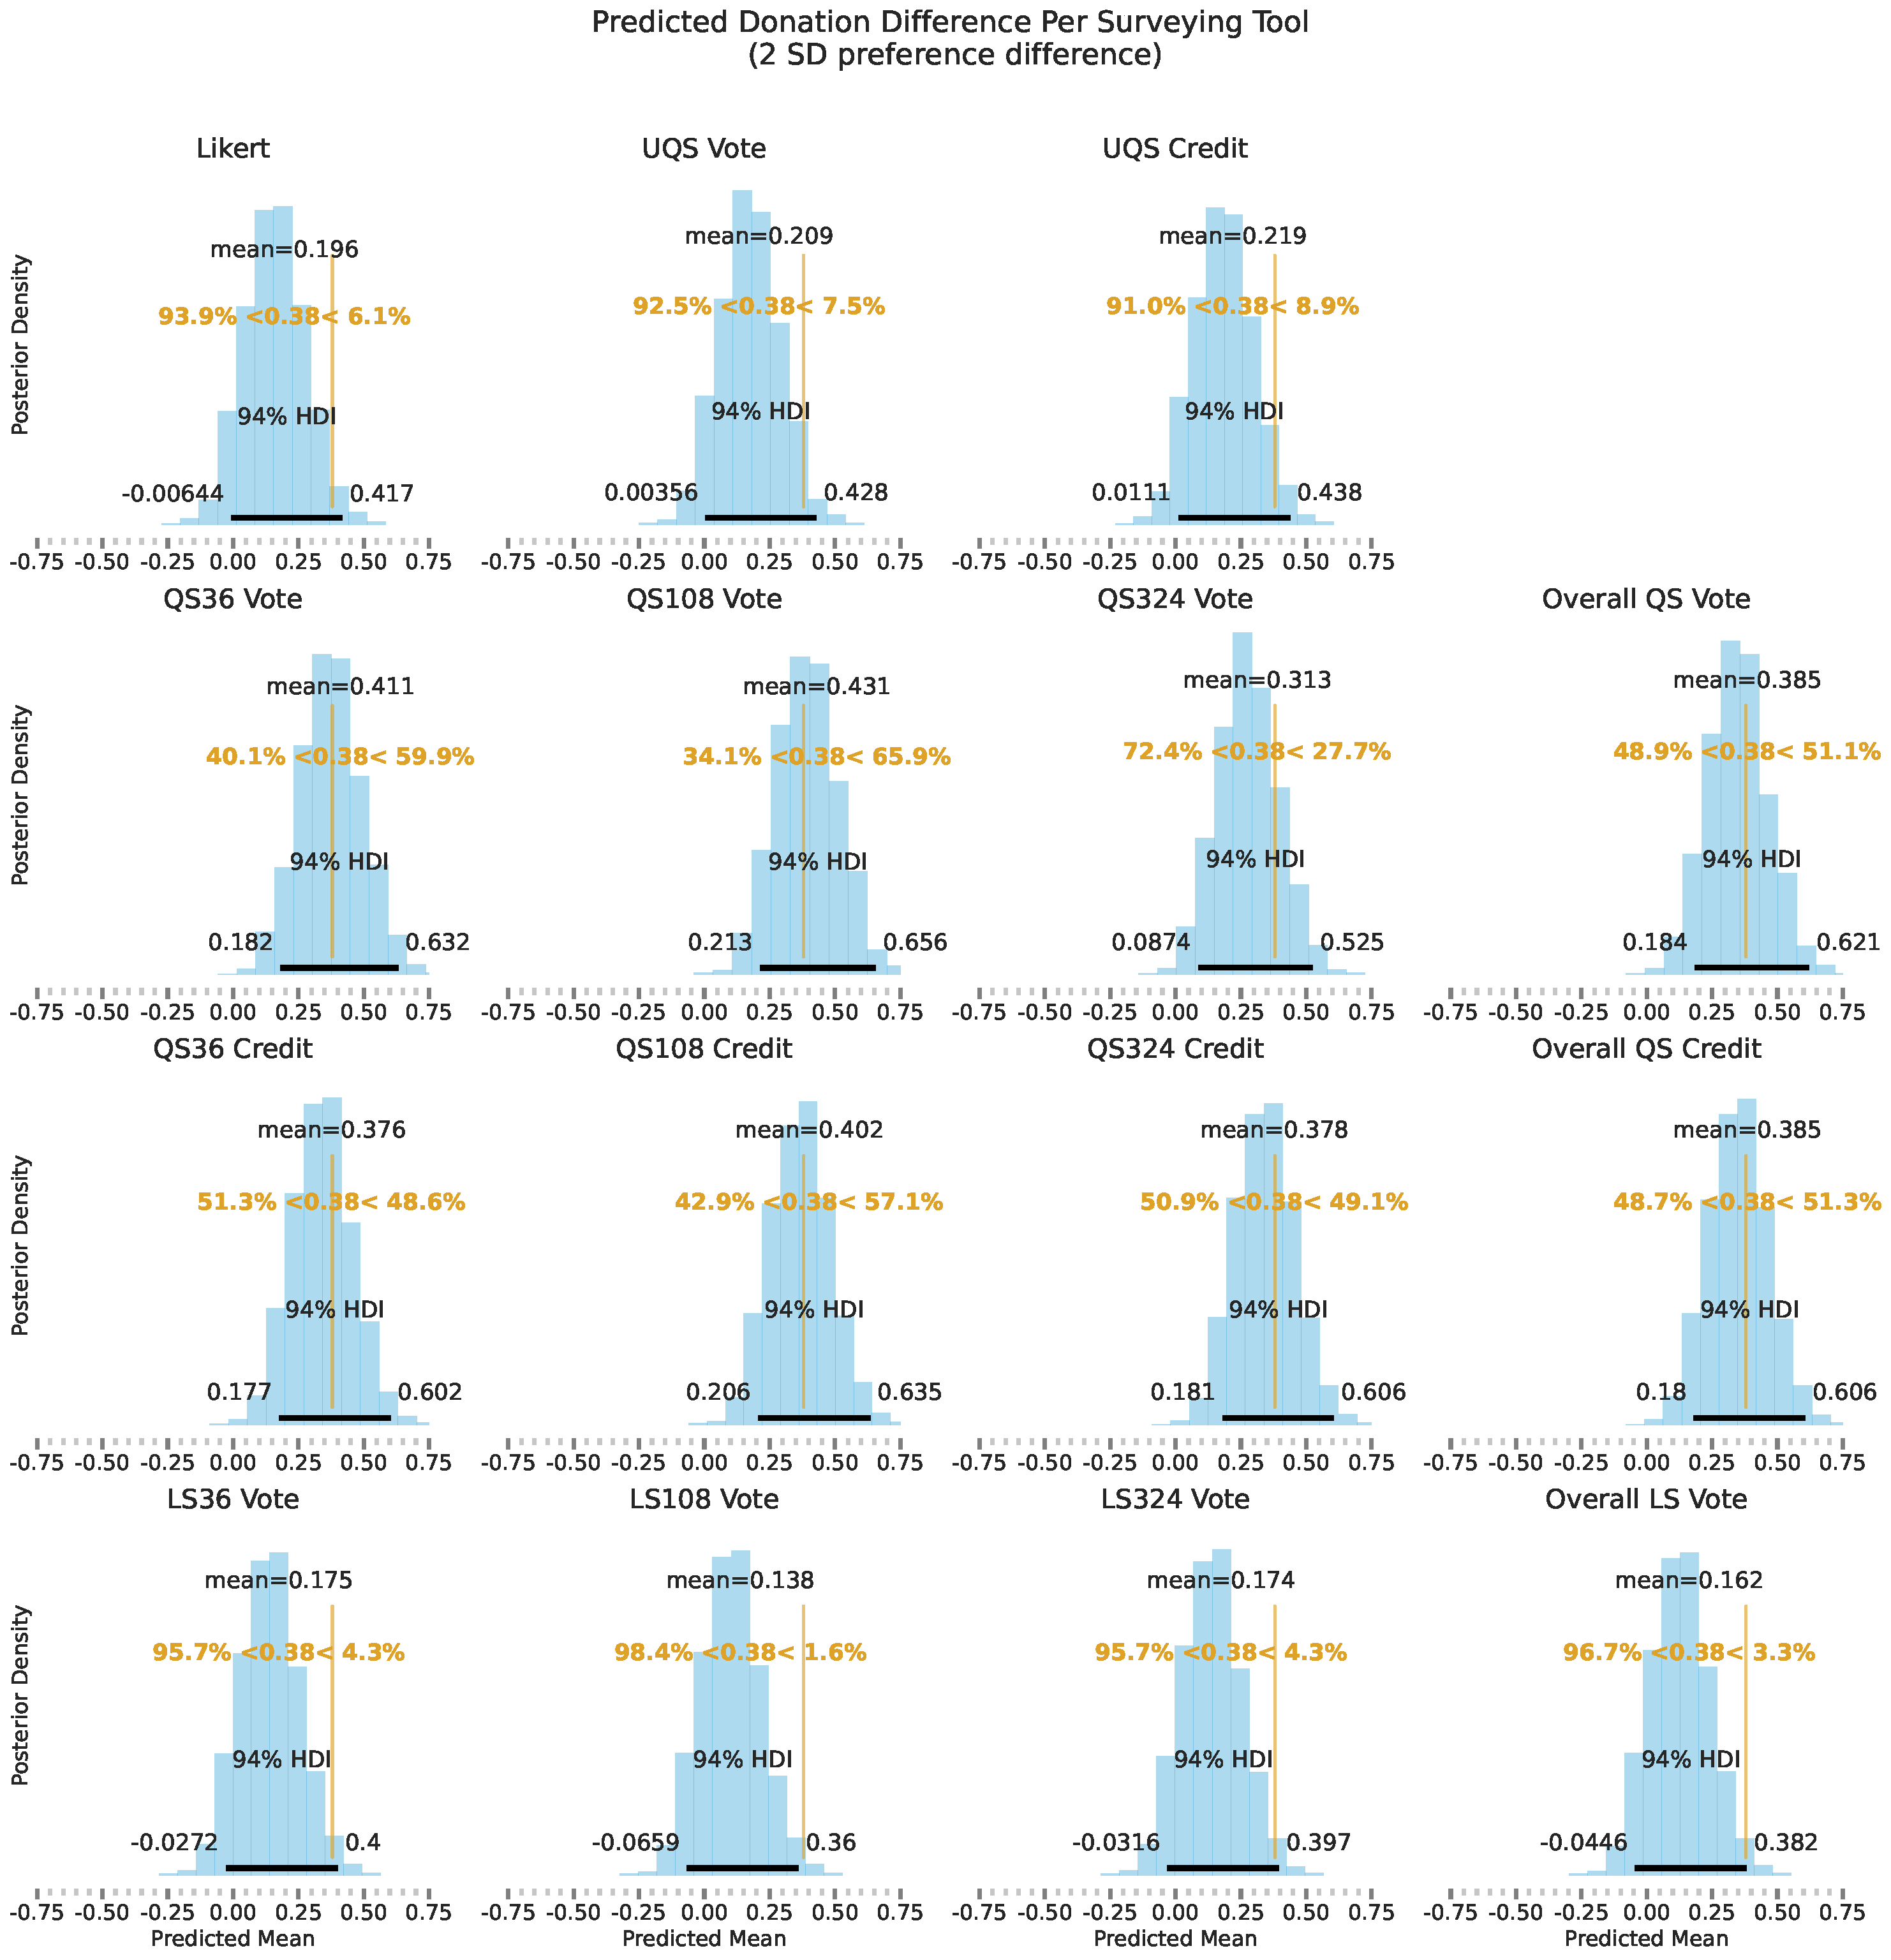
\includegraphics[width=\textwidth]{content/image/intensity_2sd.pdf}
    \caption{Comparison of preference elicitation methods: QS, LS, UQS, and Linear Survey.}
    \Description{Comparison of preference elicitation methods: QS, LS, UQS, and Linear Survey.}
    \label{fig:comparison}
\end{figure}


\textbf{Results interpretation:} With the fitted intensity model, we calculate the posterior predictive distribution of the mean of donation differences ($\mu_{\Delta_{PredictedDonation}}$), given a preference difference intensity between any two causes elicited by a survey tool ($\Delta_{Survey}$). We construct three such distributions for each survey tool, one for a small, medium, and large preference difference elicited by the tool respectively (i.e., $\Delta_{Survey}$ = 0.19, 0.38, 0.57, corresponding to $median(\Delta_{Survey})+k \times std(\Delta_{Survey})$, where $k=1, 2, 3$). We then perform two comparison tasks using these posterior distributions of $\mu_{\Delta_{PredictedDonation}}$. 

First, we evaluate if predicted normalized donation differences $\Delta_{PredictedDonation}$ significantly differ from the ``perfect'' predicted donation difference ($\Delta_{DonationRef}$). A predicted normalized donation difference between two causes is ``perfect'' when it equals the normalized difference between the preferences elicited by the survey tool ($\Delta_{DonationRef} = \Delta_{Survey}$). When $\Delta_{PredictedDonation} < \Delta_{DonationRef}$, it means that our participants donated less to their preferred cause than they said they would on the survey (relative to the less-preferred cause), and vice-versa. We conclude that a survey tool failed to reflect a given preference difference intensity well when the 94\% Highest Posterior Density Interval (HPDI) of the distribution of $\mu_{\Delta_{PredictedDonation}}$ does not include $\Delta_{DonationRef}$. 

Second, we compare the posterior distributions of $\mu_{\Delta_{PredictedDonation}}$ between survey conditions for the same $\Delta_{Survey}$. Such comparisons provide insights into how a survey tool performs relative to another. We construct the posterior distribution of Cohen's d to quantify the difference between the $\mu_{\Delta_{PredictedDonation}}$ of a pair of survey conditions. We report that a survey tool's ability to reflect a preference intensity differs from another when the 94\% HPDI of the Cohen's d distribution excludes zero. 

\textbf{Small $\Delta_{Survey}$ in all tested survey tools predicted $\Delta_{PredictedDonation}$ well.} Among them, Likert, UQS vote, UQS credit, and LS results aligned best with donation differences (mean of $\mu_{\Delta_{PredictedDonation}}$ = 0.15, 0.17, 0.18, 0.15, respectively; $\Delta_{DonationRef}$ = 0.19). When participants expressed a small difference in QS vote and credit between two causes, they expressed larger differences in donations (mean of $\mu_{\Delta_{PredictedDonation}}$ = 0.29, 0.26, respectively). But their donation differences did not differ significantly from the ``perfect'' difference ($\Delta_{DonationRef}$ = 0.19).

\textbf{As $\Delta_{Survey}$ increased to medium and large sizes, only those elicited by QS (both vote and credit, regardless of the budget size) were well-reflected in the corresponding donation differences.} For instance, when QS vote and credit $\Delta_{Survey} = 0.38$ (medium difference), the mean of $\mu_{\Delta_{PredictedDonation}} = 0.39$ (94\% HPDI for QS vote = [0.18, 0.62], for QS credit = [0.18, 0.61]). \textbf{Results from QS aligned significantly better with donation results than those from the Likert scale with a medium to large effect size}\footnote{Cohen's d = 0.2, 0.5, 0.8 corresponds to a small, medium, and large effect size, respectively}. Moreover, QS's advantage over the Likert scale increased with $\Delta_{Survey}$, as shown in Figure~\ref{fig:comparison}. Using the donation prediction accuracy of QS credit vs. Likert scale as an example, the mean Cohen's d increases from 0.71 to 0.99 when $\Delta_{Survey}$ changes from medium (Cohen's d 94\% HPDI = [0.62, 0.81]) to large (Cohen's d 94\% HPDI = [0.89, 1.09]).

\textbf{On the other hand, for medium and large $\Delta_{Survey}$, UQS (i.e., QS without a budget) predicted donation difference similarly to the Likert scale, hence significantly worse than QS. Furthermore, LS with various budget sizes (i.e., QS without the quadratic cost) performed worse than Likert and UQS with a small effect size.} When participants conveyed a medium-sized or larger preference difference between two causes in Likert, UQS, or LS, they expressed a weaker difference in donations. A large $\Delta_{Survey}$ in Likert, UQS, and LS, for instance, predicted a mean $\mu_{\Delta_{PredictedDonation}}$ of 0.25, 0.25, and 0.17 respectively, far lower than the ideal difference ($\Delta_{DonationRef}$ = 0.57).

% For example, Cohen's d's mean for LS vs. Likert was -0.33 (94\% HPDI = [-0.45, -0.21]) when $\Delta_{Survey} = 0.57$ (large difference). 